% Auto-generated by paper/figures/build_results_package.py
% Drop-in snippet for the Split-CIFAR-100 results section.

\begin{table}[t]
  \centering
  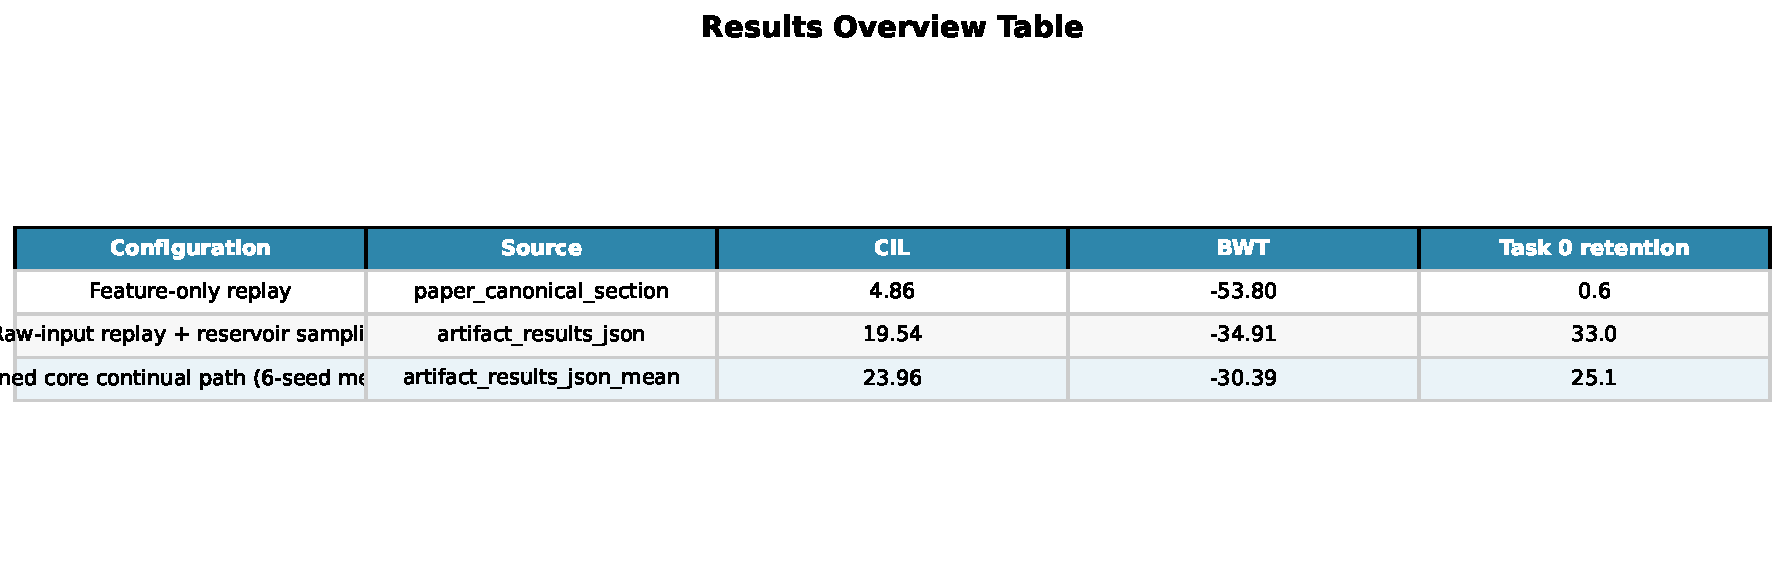
\includegraphics[width=\linewidth]{../figures/generated/results_package/table_results_overview.pdf}
  \caption{Split-CIFAR-100 continual-learning progression. Phase 1 is a legacy feature-only replay result sourced from the canonical paper section because the original run directory is not currently tracked as a local artifact. Phase 2 and Phase 3 are artifact-backed, with Phase 3 reporting the mean over 6 tuned-core Titan runs from family `20260311_140818`.}
  \label{tab:split-cifar-results-overview}
\end{table}

\begin{figure}[t]
  \centering
  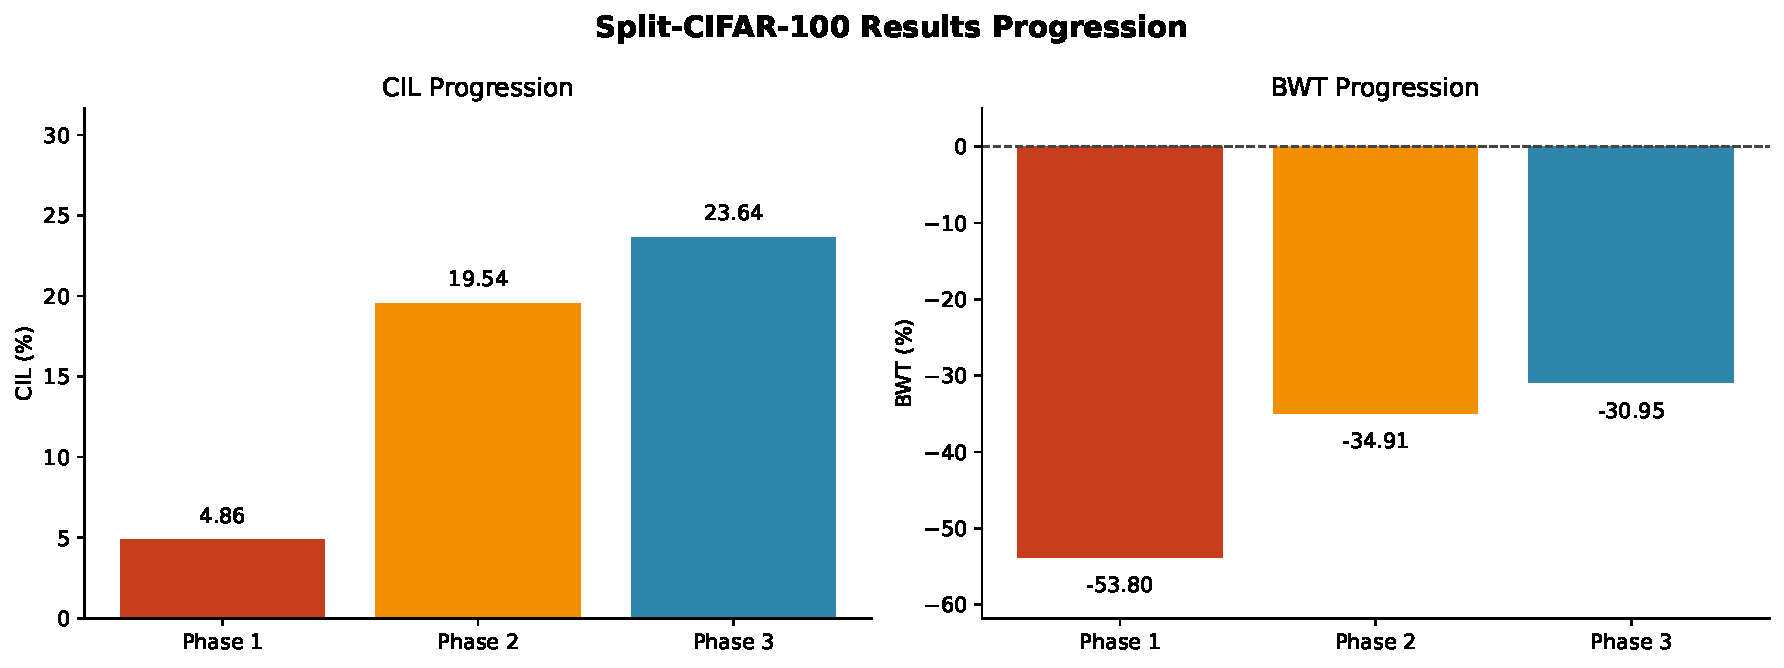
\includegraphics[width=\linewidth]{../figures/generated/results_package/figure_phase_progression.pdf}
  \caption{CIL and BWT progression from feature-only replay to raw-input replay with reservoir sampling and then the tuned-core continual configuration. The figure emphasizes that replay-path design, not just stronger regularization, drove the major retention gains.}
  \label{fig:split-cifar-phase-progression}
\end{figure}

\begin{figure}[t]
  \centering
  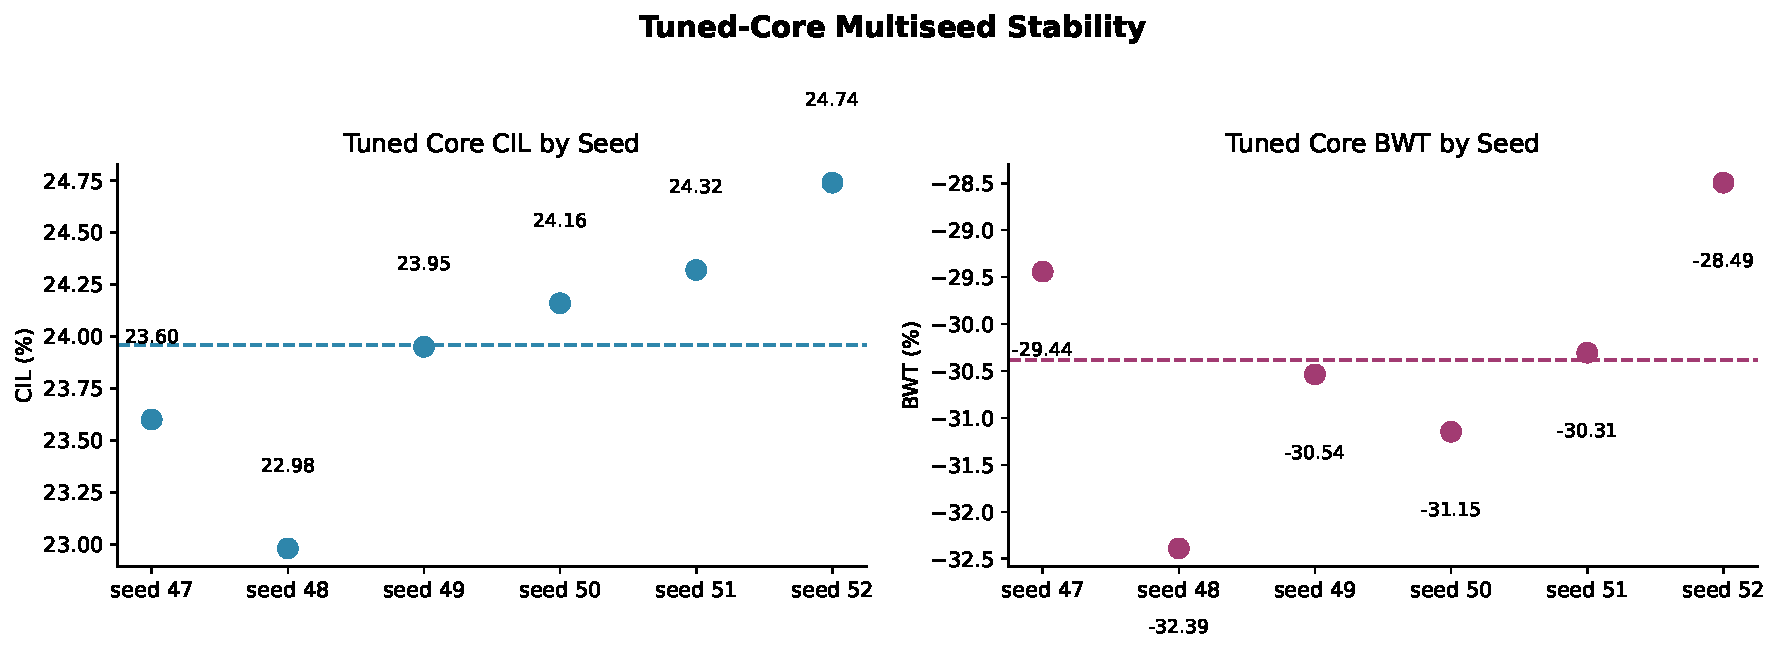
\includegraphics[width=\linewidth]{../figures/generated/results_package/figure_tuned_core_multiseed.pdf}
  \caption{Tuned-core multiseed stability on Titan Node. Each point is one full 20-task Split-CIFAR-100 run, with dashed lines indicating the multiseed means. Variance is modest relative to the mean effect size.}
  \label{fig:tuned-core-multiseed}
\end{figure}

\begin{figure}[t]
  \centering
  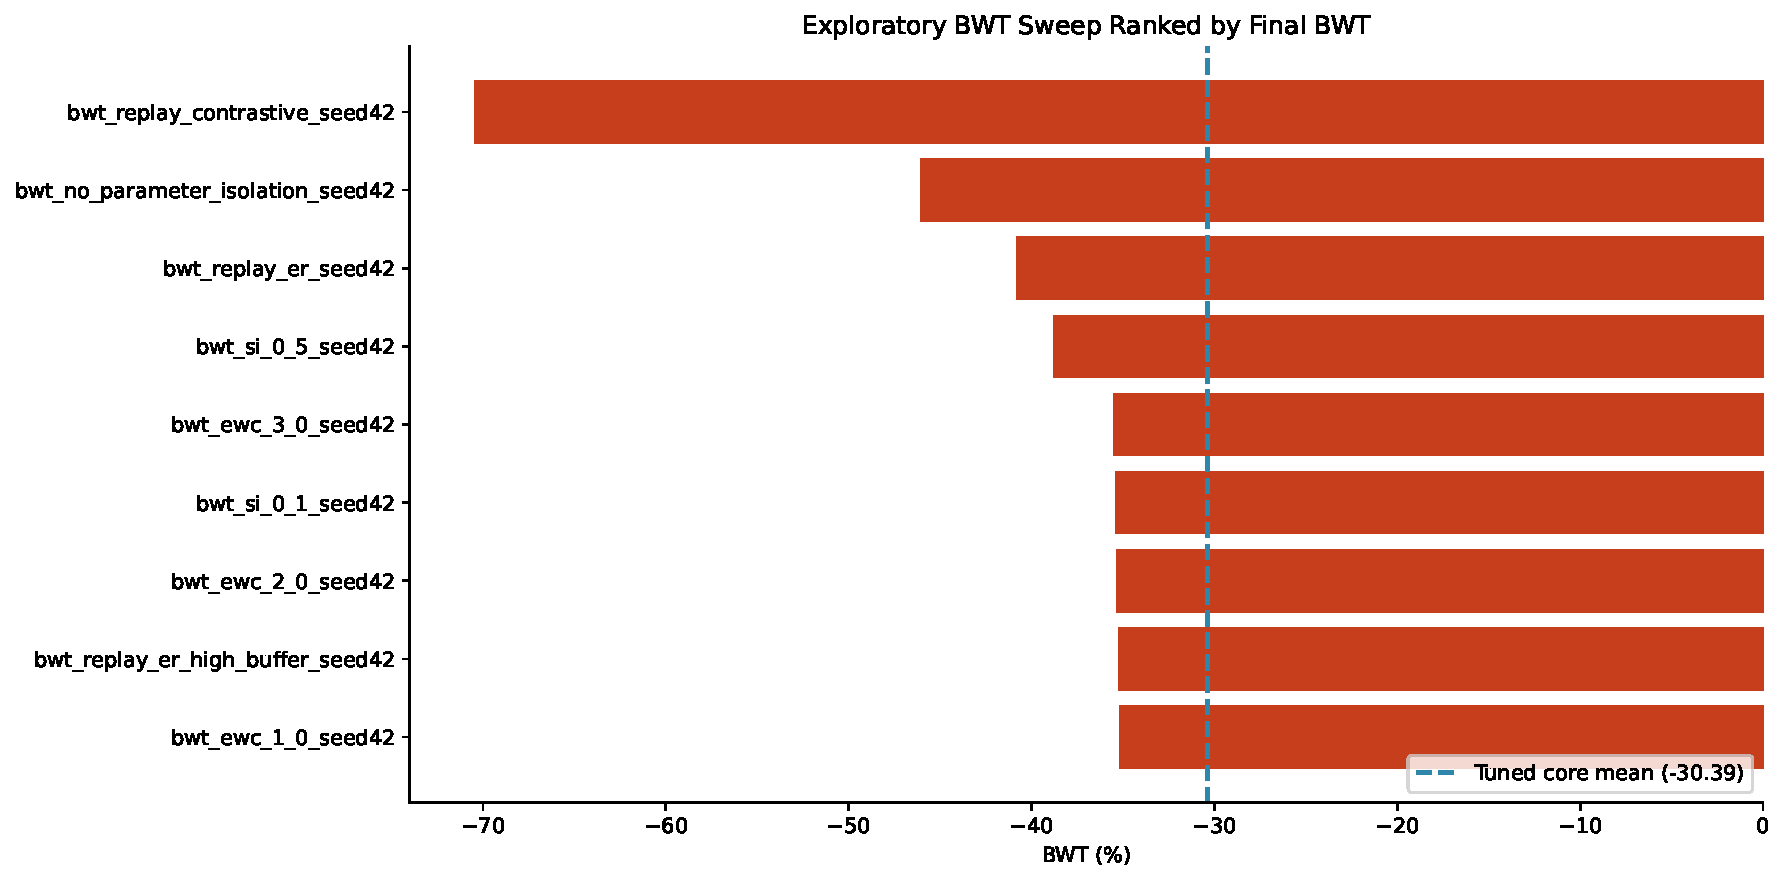
\includegraphics[width=\linewidth]{../figures/generated/results_package/figure_bwt_sweep_ranked.pdf}
  \caption{Exploratory BWT sweep ranked by final BWT. The dashed reference line marks the tuned-core multiseed mean. None of the completed EWC, SI, larger-buffer ER, or contrastive replay runs surpass the tuned-core baseline.}
  \label{fig:bwt-sweep-ranked}
\end{figure}

\begin{figure}[t]
  \centering
  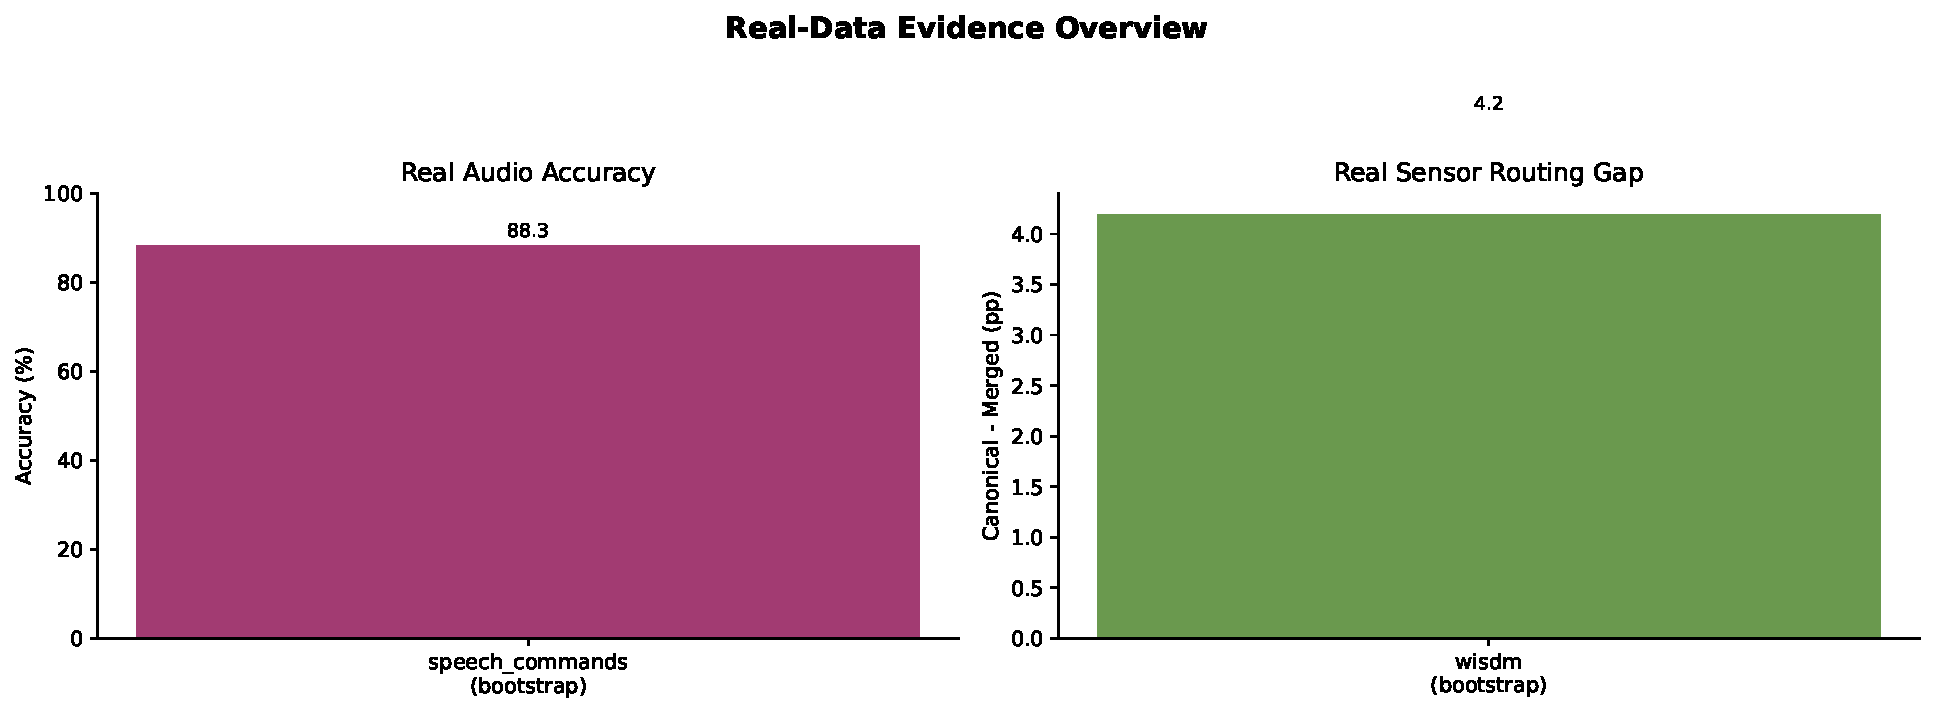
\includegraphics[width=\linewidth]{../figures/generated/results_package/figure_real_data_evidence.pdf}
  \caption{Real-data evidence overview. Bootstrap evidence comes from `real-audio-seq-001` on Speech Commands and `real-seq-004` on WISDM. Canonical evidence is promoted from `real-audio-seq-002` and `real-sensor-seq-001` as those bounded integrated sequences complete. Historical bootstrap reports may still list newly integrated datasets as candidates, so the package treats sequence stage and current supervisor defaults as the canonical source of truth.}
  \label{fig:real-data-evidence-overview}
\end{figure}
